\chapter{Исследовательская часть}

\section{Технические характеристики}

Технические характеристики устройства, на котором выполнялись замеры по времени представлены далее.

\begin{itemize}
	\item Процессор: Intel(R) Core(TM) i5-10300H CPU @ 2.50 ГГц 2.50 ГГц.
	\item Оперативная память: 16 ГБ.
	\item Операционная система: Windows 10 Pro 64-разрядная система версией 21H2.
\end{itemize}

При замерах времени ноутбук был включен в сеть электропитания и был нагружен только системными приложениями.

\section{Демонстрация работы программы}

\begin{figure}[h]
	\centering
	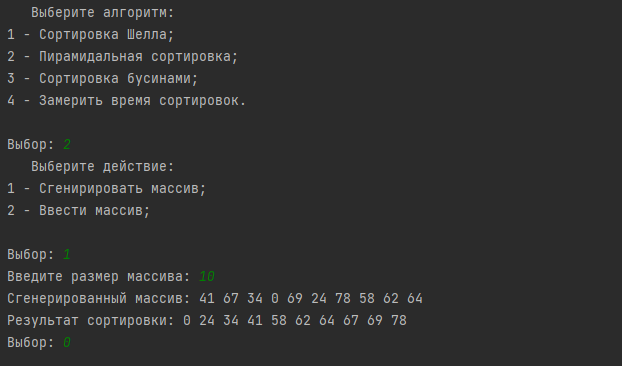
\includegraphics[height=0.4\textheight]{img/example.png}
	\caption{Демонстрация работы программы}
	\label{img:demonstration}
\end{figure}

\clearpage

\section{Временные характеристики}

Результаты эксперимента замеров по времени приведены в Таблицах \ref{tbl:time_sort}, \ref{tbl:time_random}, \ref{tbl:time_rsort}.

В Таблице \ref{tbl:time_sort} приведены результаты замеров по времени лучшего случая для сортировки Шелла и пирамидальной сортировки, то есть это отсортированный массив данных по возрастанию. Лучшим случаем для сортировки Бусинами является массив с элементами минимального значения.

\begin{table}[ht]
	\small
	\begin{center}
		\caption{Замеры по времени лучшего случая для сортировок, размер которых от 50 до 1000.}
		\label{tbl:time_sort}
		\begin{tabular}{|c|c|c|c|}
			\hline
			& \multicolumn{3}{c|}{\bfseries Время, мс} \\ \cline{2-4}
			\bfseries Количество элементов & \bfseries Шелла & \bfseries Пирамидальный & \bfseries Бусинами
			\csvreader{csv/sort_time.csv}{}
			{\\\hline \csvcoli & \csvcolii & \csvcoliii & \csvcoliv} \\
			\hline
		\end{tabular}
	\end{center}
\end{table}

По таблице \ref{tbl:time_sort} был построен графики \ref{plt:sort_1} и \ref{plt:sort_2}. Исходя из этих данных можно понять, что лучшего всего в этом случае работает сортировка Шелла. При этом разница во времени между пирамидальной сортировкой и сортировкой Шелла незначительна в 2 раза, а худшего всего работает сортировка бусинами в 100-200 раз, чем остальные сортировки.

\begin{figure}[h]
	\centering
	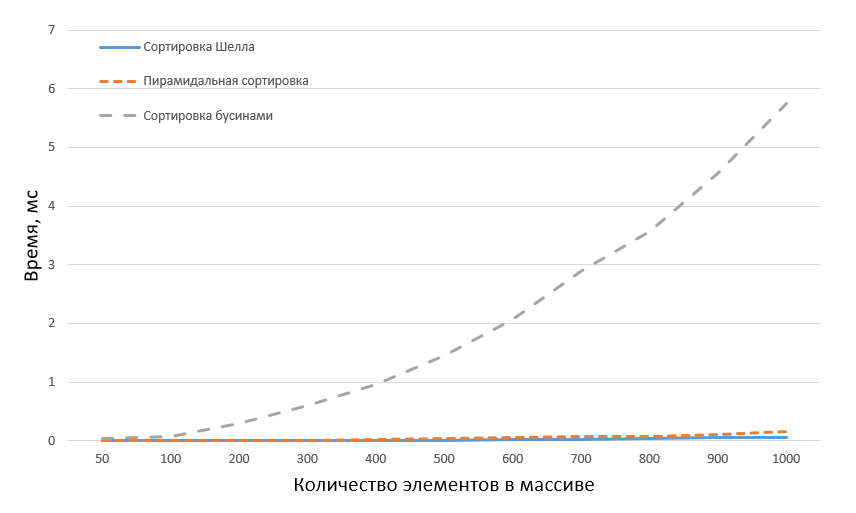
\includegraphics[height=0.3\textheight]{img/sort_1.png}
	\caption{Сравнение по времени сортировок Шелла, пирамидальную и бусинами с входным отсортированным массиве по возрастанию}
	\label{plt:sort_1}
\end{figure}

\begin{figure}[h]
	\centering
	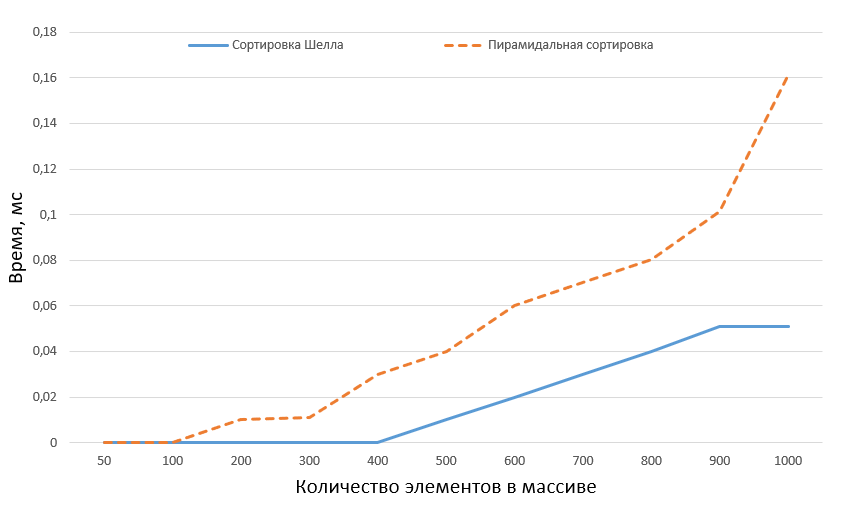
\includegraphics[height=0.3\textheight]{img/sort_2.png}
	\caption{Сравнение по времени сортировок Шелла и пирамидальную с входным отсортированным массиве по возрастанию}
	\label{plt:sort_2}
\end{figure}

\clearpage

В Таблице \ref{tbl:time_random} приведены результаты замеров по времени для сортировки Шелла, пирамидальной сортировки и сортировки бусинами, где на вход поступает случайный массив данных.

\begin{table}[ht]
	\small
	\begin{center}
		\caption{Замеры по времени, размер которых от 50 до 1000, с входным случайным массивом}
		\label{tbl:time_random}
		\begin{tabular}{|c|c|c|c|}
			\hline
			& \multicolumn{3}{c|}{\bfseries Время, мс} \\ \cline{2-4}
			\bfseries Количество элементов & \bfseries Шелла & \bfseries Пирамидальный & \bfseries Бусинами
			\csvreader{csv/sort_time.csv}{}
			{\\\hline \csvcoli & \csvcolii & \csvcoliii & \csvcoliv} \\
			\hline
		\end{tabular}
	\end{center}
\end{table}

По таблице \ref{tbl:time_random} был построен график \ref{plt:random}. Исходя из этих данных можно понять, что лучшего всего в этом случае работает сортировка Шелла. При этом разница во времени между пирамидальной сортировкой и сортировкой Шелла незначительна в 1,5 раза, а худшего всего работает сортировка бусинами в 50-100 раз, чем остальные сортировки.

\begin{figure}[h]
	\centering
	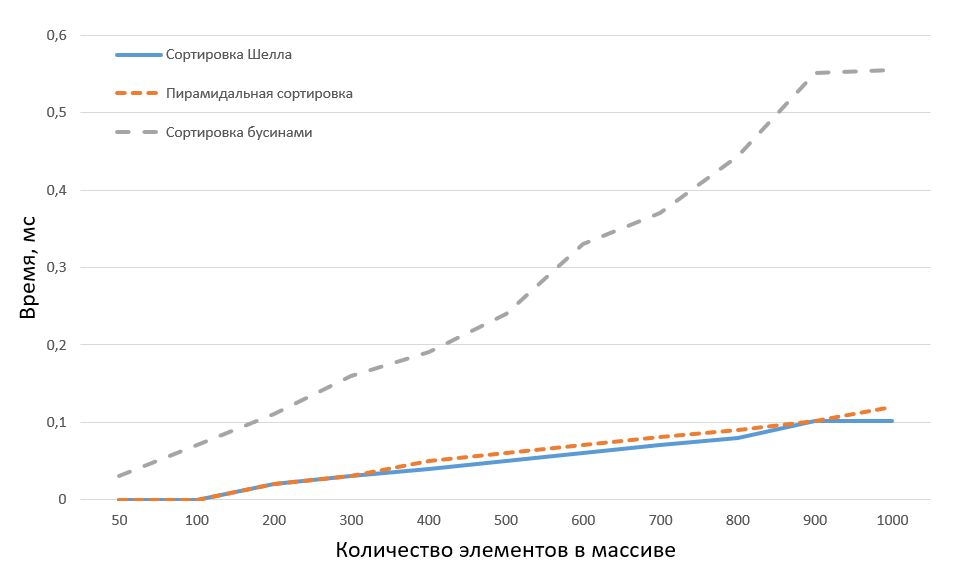
\includegraphics[height=0.3\textheight]{img/random.png}
	\caption{Сравнение по времени сортировки Шелла, пирамидальной и бусинами с входным случайным массивом}
	\label{plt:random}
\end{figure}

\clearpage

В Таблице \ref{tbl:time_rsort} приведены результаты замеров худшего случая по времени для сортировки Шелла, пирамидальной сортировки и сортировки бусинами, то есть для сортировок Шелла и пирамидальной это случаи, когда массив отсортирован по убыванию (в обратном порядке сортировки), а для сортировки бусинами учтены большие данные, так как на вход поступает массив целых чисел, то это числа больше 1000.

\begin{table}[ht]
	\small
	\begin{center}
		\caption{Замеры по времени, размер которых от 50 до 1000, с входным отсортированным массивом по убыванию}
		\label{tbl:time_rsort}
		\begin{tabular}{|c|c|c|c|}
			\hline
			& \multicolumn{3}{c|}{\bfseries Время, мс} \\ \cline{2-4}
			\bfseries Количество элементов & \bfseries Шелла & \bfseries Пирамидальный & \bfseries Бусинами
			\csvreader{csv/rsort_time.csv}{}
			{\\\hline \csvcoli & \csvcolii & \csvcoliii & \csvcoliv} \\
			\hline
		\end{tabular}
	\end{center}
\end{table}

По таблице \ref{tbl:time_random} был построен графики \ref{plt:rsort_1} и \ref{plt:rsort_2}. Исходя из этих данных можно понять, что лучшего всего в этом случае работает пирамидальная сортировка. При этом разница во времени между пирамидальной сортировкой и сортировкой Шелла незначительна в 1,5 раза, а худшего всего работает сортировка бусинами в 500 раз, чем остальные сортировки.

\begin{figure}[h]
	\centering
	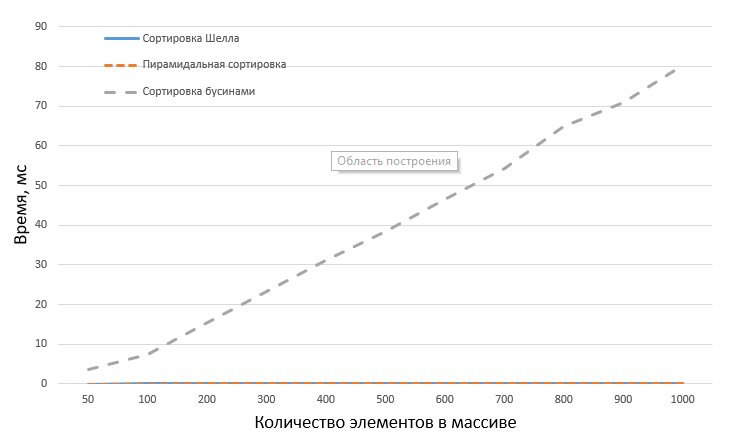
\includegraphics[height=0.3\textheight]{img/rsort_1.png}
	\caption{Сравнение по времени сортировок Шелла, пирамидальной и бусинами с входным отсортированным массивом по убыванию}
	\label{plt:rsort_1}
\end{figure}

\begin{figure}[h]
	\centering
	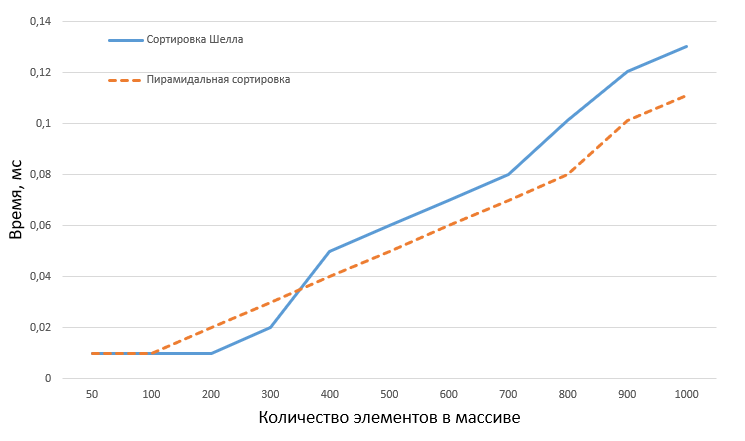
\includegraphics[height=0.3\textheight]{img/rsort_2.png}
	\caption{Сравнение по времени сортировок Шелла и пирамидальной с входным отсортированным массивом по убыванию}
	\label{plt:rsort_2}
\end{figure}

\clearpage

\section{Сравнительный анализ алгоритмов}
Приведенные временные характеристики показывают нам, что лучшей сортировкой при работе с отсортированным массивом по возрастанию является сортировка Шелла, а при работе с отсортированном массиве по убыванию (в обратном порядке для сортировки) является пирамидальная сортировка. Сортировка бусинами же показала худшие результаты по сравнению с сортировкой Шелла и пирамидальной в 50-500 раз взависимости от входных данных.

\section{Вывод}
В данном разделе было произведено сравнение количества затраченного времени вышеизложенных алгоритмов. Наименее затратным по времени оказался сортировка Шелла для отсортированного массива по возрастанию и пирамидальная сортировка для отсортированного массива по убыванию, а худшей сортировкой оказалась сортировка бусинами в сравнении с остальными сортировками.
